\subsection{Test 1}
\begin{enumerate}
	\item Consider two intersecting lines $\vec{r_1}(t)=\langle 2,3,4t\rangle$ and $\vec{r_2}(t)=\langle 2+t,3+2t,0\rangle$. Give the direction vector of each line. Find the equation of the plane which contains both lines. Draw a diagram of the lines, the plane, and the relevant vectors.\\
	\indent
	The direction vector of a line is the derivative of the position vector.
	\begin{itemize}
		\item Direction 1: $\langle 0,0,4\rangle$
		\item Direction 2: $\langle 1,2,0\rangle$
	\end{itemize}
	A the normal vector of the plane is the cross product of the direction vectors.
	\begin{itemize}
		\item $\vec{n}=\langle 0,0,4\rangle\times\langle 1,2,0\rangle=\langle -8,4,0\rangle$
	\end{itemize}
	The lines intersect when $t=0$ at $(2,3,0)$.
	So, the plane equation is: $\langle -8,4,0\rangle\cdot\langle x-2,y-3,z\rangle=0$
	
	\begin{figure}[h]
		\centering
		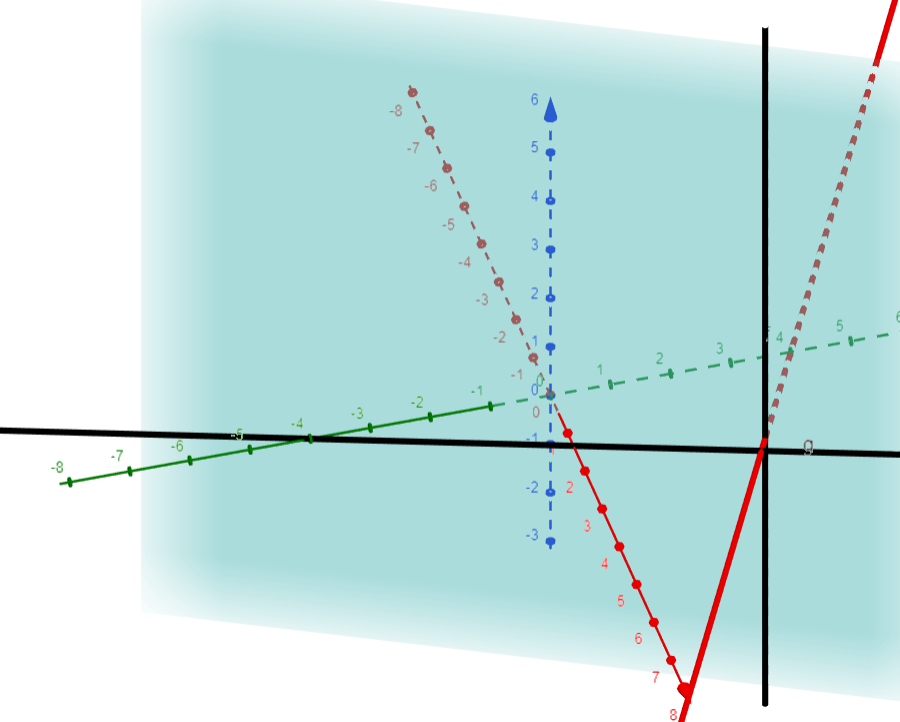
\includegraphics[scale=.5]{Images/additionalMaterials/test1_plane}
	\end{figure}
	
	\item Given the VVF $\vec{r}(t)\langle 10t, 7\cos{t}, 7\sin{t}\rangle$...\\
	\begin{enumerate}[a.]
		\item Compute the unit tangent vector $\hat{T}(t)$ and the unit normal vector $\hat{N}(t)$.\\
		\indent
		$\hat{T}=\frac{\vec{r^\prime}(t)}{\norm{\vec{r^\prime}(t)}}$\\
		$\vec{r^\prime}(t)=\langle 10,-7\sin{t},7\cos{t}\rangle$\\
		$\norm{\vec{r^\prime}(t)}=\sqrt{10^2+(-7\sin{t})^2+(7\cos{t})^2}=\sqrt{149}$\\
		$\hat{T}(t)=\frac{1}{\sqrt{149}}\langle 10,-7\sin{t},7\cos{t}$\\
		$\hat{N}(t)=\frac{\mathrm{d}\hat{T}/\mathrm{d}t}{\norm{\mathrm{d}\hat{T}/\mathrm{d}t}}$\\
		$\frac{\mathrm{d}\hat{T}}{\mathrm{d}t}=\frac{1}{\sqrt{149}}\langle 0,-7\cos{t}.-7\sin{t}\rangle$\\
		$\norm{\frac{\mathrm{d}\hat{T}}{\mathrm{d}t}}=\frac{1}{\sqrt{149}}\sqrt{(-7\cos{t})^2+(-7\sin{t})^2}=\frac{7}{\sqrt{149}}$\\
		$\hat{N}(t)=\langle 0,-\cos{t},-\sin{t}\rangle$
		
		\item Show that $\hat{T}\perp\hat{N}$ for all $t$.
		\indent
		If $\hat{T}\perp\hat{N}$, then $\hat{T}\cdot\hat{N}=0$ for all $t$.\\
		$\hat{T}\cdot\hat{N}=\frac{1}{\sqrt{149}}\langle 10, -7\sin{t}, 7\cos{t}\rangle\cdot\langle 0,-\cos{t},-\sin{t}\rangle$\\
		$=\frac{1}{\sqrt{149}}(0+7\sin{t}\cos{t}-7\sin{t}\cos{t})=0$\\
		$\implies \hat{T}\perp\hat{N}$\\
	\end{enumerate}
	
	\item A cannon fires cannonballs with a speed of $20\text{ m}/\text{s}$. Take acceleration due to gravity to be $g=10\text{m}/\text{s}^2$.
	\begin{enumerate}[a.]
		\item Starting with a constant acceleration function $\vec{a}=\langle 0,-g\rangle$, find the velocity and position functions ($\vec{r^\prime}(t)\text{ and }\vec{r}(t)$ respectively) of the cannonball if the cannon is fired from an angle $\theta$ with respect to the horizontal. Assume the cannonball is initially positioned at the origin.\\
		\indent
		We know that velocity is the integral of acceleration.\\
		$\vec{v}(t)=\vec{r^\prime}(t)=\langle c_1,c_2-gt\rangle$\\
		We are given that the initial speed is $20\text{ m}/\text{s}$ at an angle $\theta$.\\
		$\vec{v_0}=20\langle\cos{\theta},\sin{\theta}\rangle$\\
		$\vec{v}(t)=\langle 20\cos{\theta},20\sin{\theta}-gt\rangle$\\
		We know that position is the integral of velocity.\\
		$\vec{r}(t)=\langle 20t\cos{\theta}+c_1,20t\sin{theta}-\frac{1}{2}gt^2+c_2\rangle$\\
		We are given that the cannonball starts at the origin.\\
		$\vec{r}(t)=\langle 20t\cos{\theta}, 20t\sin{theta}-\frac{1}{2}gt^2\rangle$\\
		Taking $g=10\text{m}/\text{s}^2$,\\
		$\vec{r}(t)=\langle 20t\cos{\theta},20t\sin{\theta}-5t^2\rangle$\\
			
		\item What angle $\theta$ should the cannon be fired to hit a target on the ground at a distance $40\text{ m}$ away?\\
		\indent
		We want to find a point on the trajector where $y=0$ and $x=40$.
		$y=0$ when $t=0,4\sin{\theta}$. We can reasonable eliminate $t=0$ because this is when the cannon first fires and $x=0$.\\
		Plugging in $t=4\sin{\theta}$ to the x-component of position when $x=40$,\\
		$20\cos{\theta}\cdot 4\sin{\theta}=40$\\
		$2\sin{\theta}\cos{\theta}=1$\\
		$\sin{(2\theta)}=1, 2\theta=\pi/2$\\
		$\implies \theta=\pi/4$\\
	\end{enumerate}
	
	\item Consider the following particle trajectory: $\vec{r}(t)=\langle R\cos{e^t},R\sin{e^t},\frac{h}{2\pi}e^t\rangle$ for $t\geq 0$. The shape of the trajectory is a helix with radius $R$ and vertical spacing $h$. Find the arc length function $s(t)$ of the trajectory starting with $s(0)=0$. Give the arc length reparameterization of the helix.\\
	\indent
	$s(t)=\int_{0}^{t}{\norm{\vec{r^\prime}(\tau)}\mathrm{d}\tau}$\\
	$\vec{r^\prime}(t)=\langle -Re^{t}\sin{e^t},Re^{t}\cos{e^t},\frac{h}{2\pi}e^{t}\rangle$\\
	$\norm{\vec{r^\prime}(t)}=\sqrt{(-Re^{t}\sin{e^t})^2+(Re^{t}\cos{e^t})^2+(\frac{h}{2\pi}e^t)^2}$\\
	$=e^{t}\sqrt{R^2+\frac{h^2}{4\pi^2}}$\\
	$s(t)=\int_{0}^{t}{e^{\tau}\sqrt{R^2+\frac{h^2}{4\pi^2}}\mathrm{d}\tau}=\sqrt{R^2+\frac{h^2}{4\pi^2}(e^{t}-1)}$\\
	Solving for $t$,\\
	$t=\ln{\left(\frac{s}{\sqrt{R^2+\frac{h^2}{4\pi^2}}}+1\right)}$\\
	$\vec{r}(s)=\left<R\cos{\left(\frac{s}{\sqrt{R^2+\frac{h^2}{4\pi^2}}}+1\right)},R\sin{\left(\frac{s}{\sqrt{R^2+\frac{h^2}{4\pi^2}}}+1\right)},\frac{h}{2\pi}\left(\frac{s}{\sqrt{R^2+\frac{h^2}{4\pi^2}}}+1\right)\right>$\\
	
	\item Let $\vec{r}(t)$ be the position function of a particle trapped on the surface of a sphere centered at the origin. Show that $\vec{r}(t)\perp\frac{\mathrm{d}}{\mathrm{d}t}\vec{r}(t)$ for all $t$.\\
	\indent
	Since $\vec{r}(t)$ is on a sphere, $\norm{\vec{r}(t)}=R$ and $\vec{r}(t)\cdot\vec{r}(t)=R^2$.\\
	$\frac{\mathrm{d}}{\mathrm{d}t}(\vec{r}(t)\cdot\vec{r}(t))=2\vec{r}(t)\cdot\vec{r^\prime}(t)$\\
	$\frac{\mathrm{d}}{\mathrm{d}t}(\vec{r}(t)\cdot\vec{r}(t))=\frac{\mathrm{d}}{\mathrm{d}t}R^2=0$\\
	So, $2\vec{r}(t)\cdot\vec{r^\prime}(t)=0$ and $\vec{r}(t)\cdot\vec{r^\prime}(t)=0$\\
	$\implies\vec{r}(t)\perp\vec{r^\prime}(t)$\\
\end{enumerate}